\input{preamble.tex}
\newcommand{\C}{\mathcal{C}}
\pgfplotsset{tick style={very thin}} 



\begin{document}
\pagestyle{fancy}
\fancyhead[L]{Seconde}
\fancyhead[C]{\textbf{Evaluation flash n°5a}}
\fancyhead[R]{\today}

\reversemarginpar

\null\vspace{-30pt}
Nom / Prénom : \\

Consignes particulières : 
\begin{itemize}[label=$\bullet$]
	\item 
	La calculatrice est \textbf{interdite}.
	\item
	Attention le sujet est \textbf{recto-verso}.
	\item
	Le devoir peut être réalisé entièrement sur cette feuille.
%	\item 
%	Le devoir peut être fait entièrement sur cette feuille.
%	\item 
%	Toute trace de recherche est prise en compte.
	%\item 
	%L'abbréviation $\tq$ signifie ``tel que''.
\end{itemize}

\hrule

\exe{2}{
On considère la fonction affine $f$ d'expression algébrique $f(x)=2x+3$.
Représenter la courbe $\C_f$ dans le repère ci-dessous puis compléter le tableau de signe qui suit.
	\begin{center}
	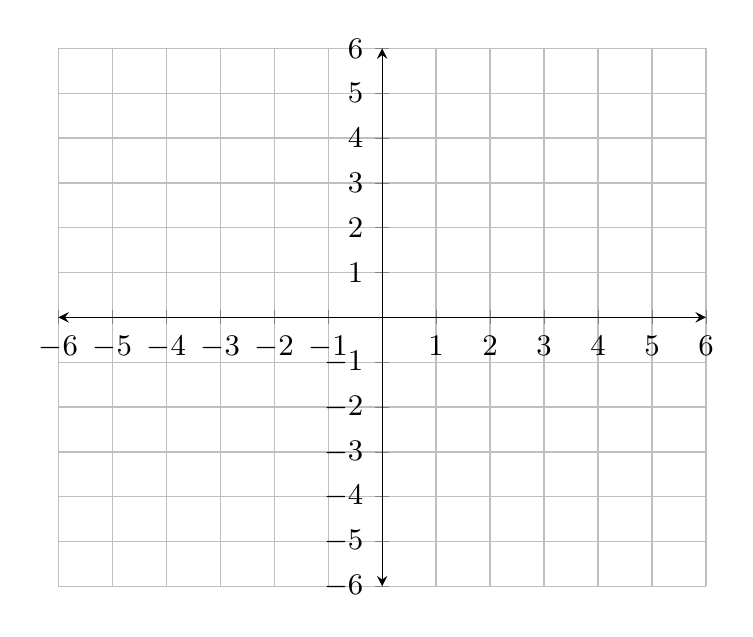
\begin{tikzpicture}[>=stealth, scale=1.2, every node/.append style={font=\small}]
	\begin{axis}[xmin = -6, xmax=6, ymin=-6, ymax=6, axis x line=middle, axis y line=middle, axis line style=<->, xlabel={}, ylabel={}, xtick = {-6, -5, ..., 5, 6}, ytick = {-6, -5, ..., 5, 6}, grid=both]
	
	\end{axis}
	\end{tikzpicture}
	
	\renewcommand\arraystretch{1.8}
	\begin{tabular}{ | c || c |}
	\cline{1-2}
	$x$ & \hspace{5cm}  \\ \hline  
	Signe de $f(x)$ & \hspace{5cm} \\ \hline
	\end{tabular}
	
	\end{center}
}{exe:1a}{

}

\exe{4}{

Compléter les tableaux de signes ci-dessous :

\begin{center}

\renewcommand\arraystretch{1.8}
\begin{tabular}{ | c || c |}
	\cline{1-2}
	$x$ & \hspace{5cm}  \\ \hline  
	Signe de $3x+5$ & \hspace{8cm} \\ \hline
	Signe de $-x+5$ & \hspace{8cm} \\ \hline
	Signe de $(3x+5)\cdot(-x+5)$ & \hspace{8cm} \\ \hline
\end{tabular}

\vspace{1cm}

\begin{tabular}{ | c || c |}
	\cline{1-2}
	$x$ & \hspace{5cm}  \\ \hline  
	Signe de $-\frac12 x+2$ & \hspace{8cm} \\ \hline
	Signe de $4x+1$ & \hspace{8cm} \\ \hline
	Signe de $(-\frac12 x+2)\cdot(4x+1)$ & \hspace{8cm} \\ \hline
\end{tabular}
\end{center}

}{exe:2a}{

}

\newpage

\exe{4}{

En vous appuyant sur la représentation graphique ci-dessous, compléter le tableau de signe qui suit.

\begin{center}
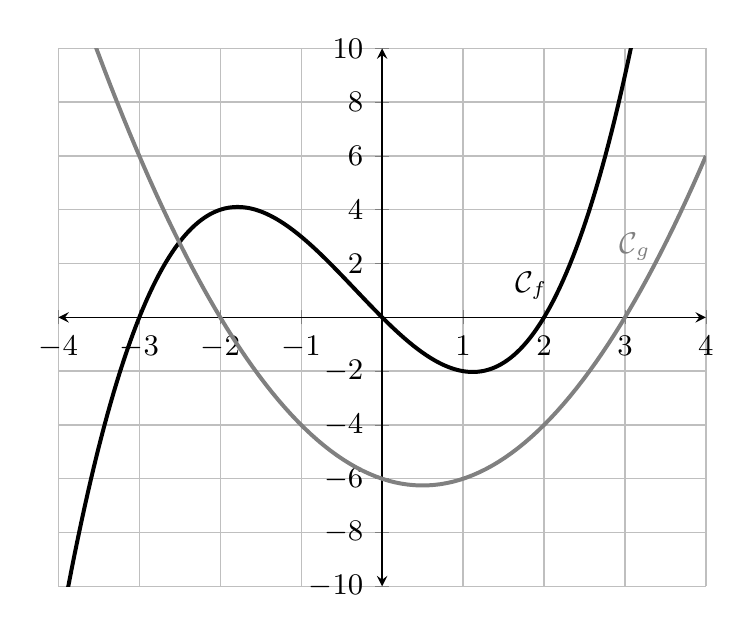
\begin{tikzpicture}[>=stealth, scale=1.2, every node/.append style={font=\small}]
	\begin{axis}[xmin = -4, xmax=4, ymin=-10, ymax=10, axis x line=middle, axis y line=middle, axis line style=<->, xlabel={}, ylabel={}, xtick = {-4, -3, ..., 3, 4}, ytick = {-10, -8, ..., 8, 10}, grid=both]

	\addplot[no marks, black, -, very thick] expression[domain=-4:4, samples=200]{(x-2)*(x+3)*x/2}
			node[pos=.5, left]{$\mathcal{C}_f$};
	\addplot[no marks, gray, -,  very thick] expression[domain=-4:4, samples=101]{(x+2)*(x-3)}
			node[pos=.9, left]{$\mathcal{C}_g$};
		\end{axis}
\end{tikzpicture}

\renewcommand\arraystretch{1.8}
\begin{tabular}{ | c || c |}
	\cline{1-2}
	$x$ & \hspace{5cm}  \\ \hline  
	Signe de $f(x)$ & \hspace{8cm} \\ \hline
	Signe de $g(x)$ & \hspace{8cm} \\ \hline
	Signe de $f(x)\cdot g(x)$ & \hspace{8cm} \\ \hline
\end{tabular}

\end{center}
}{exe:3a}{

}

\newpage

\setcounter{Exercise}{0}
\setcounter{page}{1}

\pagestyle{fancy}
\fancyhead[L]{Seconde}
\fancyhead[C]{\textbf{Evaluation flash n°5b}}
\fancyhead[R]{\today}

\reversemarginpar

\null\vspace{-30pt}
Nom / Prénom : \\

Consignes particulières : 
\begin{itemize}[label=$\bullet$]
	\item 
	La calculatrice est \textbf{interdite}.
	\item
	Attention le sujet est \textbf{recto-verso}.
	\item
	Le devoir peut être réalisé entièrement sur cette feuille.
%	\item 
%	Le devoir peut être fait entièrement sur cette feuille.
%	\item 
%	Toute trace de recherche est prise en compte.
	%\item 
	%L'abbréviation $\tq$ signifie ``tel que''.
\end{itemize}

\hrule

\exe{2}{
On considère la fonction affine $f$ d'expression algébrique $f(x)=3x-4$.
Représenter la courbe $\C_f$ dans le repère ci-dessous puis compléter le tableau de signe qui suit.
	\begin{center}
	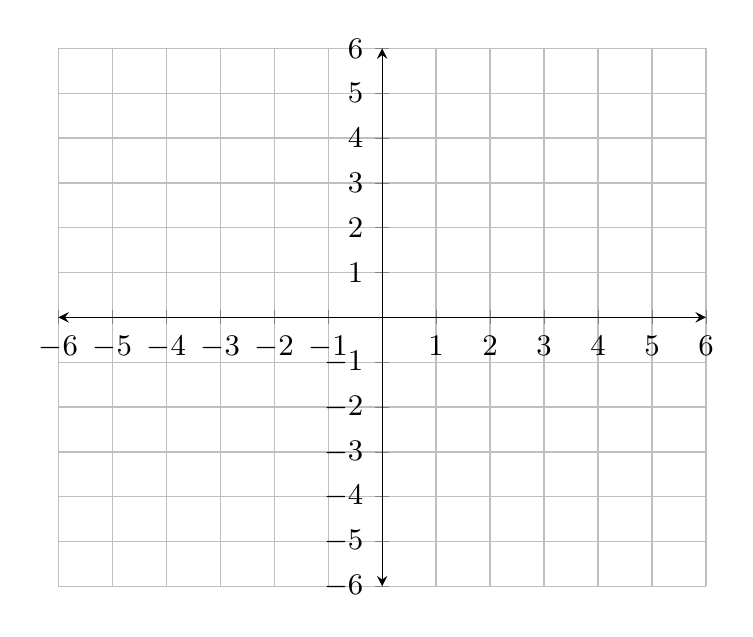
\begin{tikzpicture}[>=stealth, scale=1.2, every node/.append style={font=\small}]
	\begin{axis}[xmin = -6, xmax=6, ymin=-6, ymax=6, axis x line=middle, axis y line=middle, axis line style=<->, xlabel={}, ylabel={}, xtick = {-6, -5, ..., 5, 6}, ytick = {-6, -5, ..., 5, 6}, grid=both]
	
	\end{axis}
	\end{tikzpicture}
	
	\renewcommand\arraystretch{1.8}
	\begin{tabular}{ | c || c |}
	\cline{1-2}
	$x$ & \hspace{5cm}  \\ \hline  
	Signe de $f(x)$ & \hspace{5cm} \\ \hline
	\end{tabular}
	
	\end{center}
}{exe:1b}{

}

\exe{4}{

Compléter les tableaux de signes ci-dessous :

\begin{center}

\renewcommand\arraystretch{1.8}
\begin{tabular}{ | c || c |}
	\cline{1-2}
	$x$ & \hspace{5cm}  \\ \hline  
	Signe de $-2x+3$ & \hspace{8cm} \\ \hline
	Signe de $x+5$ & \hspace{8cm} \\ \hline
	Signe de $(-2x+3)\cdot(x+5)$ & \hspace{8cm} \\ \hline
\end{tabular}

\vspace{1cm}

\begin{tabular}{ | c || c |}
	\cline{1-2}
	$x$ & \hspace{5cm}  \\ \hline  
	Signe de $\frac12 x+2$ & \hspace{8cm} \\ \hline
	Signe de $-4x+1$ & \hspace{8cm} \\ \hline
	Signe de $(\frac12 x+2)\cdot(-4x+1)$ & \hspace{8cm} \\ \hline
\end{tabular}
\end{center}

}{exe:2b}{

}

\newpage

\exe{4}{

En vous appuyant sur la représentation graphique ci-dessous, compléter le tableau de signe qui suit.

\begin{center}
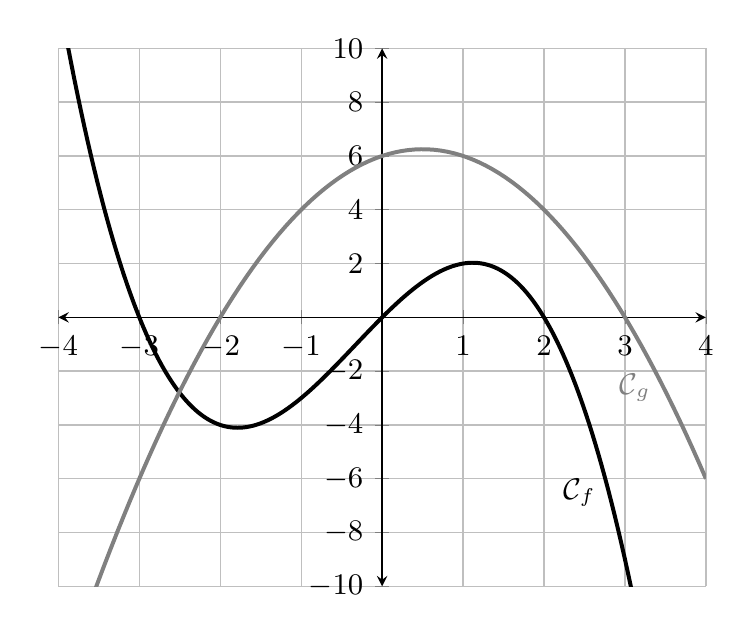
\begin{tikzpicture}[>=stealth, scale=1.2, every node/.append style={font=\small}]
	\begin{axis}[xmin = -4, xmax=4, ymin=-10, ymax=10, axis x line=middle, axis y line=middle, axis line style=<->, xlabel={}, ylabel={}, xtick = {-4, -3, ..., 3, 4}, ytick = {-10, -8, ..., 8, 10}, grid=both]

	\addplot[no marks, black, -, very thick] expression[domain=-4:4, samples=200]{-(x-2)*(x+3)*x/2}
			node[pos=.6, left]{$\mathcal{C}_f$};
	\addplot[no marks, gray, -,  very thick] expression[domain=-4:4, samples=101]{-(x+2)*(x-3)}
			node[pos=.9, left]{$\mathcal{C}_g$};
		\end{axis}
\end{tikzpicture}

\renewcommand\arraystretch{1.8}
\begin{tabular}{ | c || c |}
	\cline{1-2}
	$x$ & \hspace{5cm}  \\ \hline  
	Signe de $f(x)$ & \hspace{8cm} \\ \hline
	Signe de $g(x)$ & \hspace{8cm} \\ \hline
	Signe de $f(x)\cdot g(x)$ & \hspace{8cm} \\ \hline
\end{tabular}

\end{center}

}{exe:3b}{

}


%%%%%%%%%%%%
%
%\newpage
%\fancyhead[C]{\textbf{Solutions}}
%\shipoutAnswer

\end{document}
 